\documentclass{article}

\usepackage{graphicx} % Required for inserting images
\usepackage[spanish]{babel}
\usepackage{amsmath}
\usepackage{amssymb}
\usepackage{graphicx}
\usepackage{url}
\usepackage{times} 
\usepackage{hyperref}
\newcommand{\R}{\ensuremath{\mathbb{R}}}

\title{Tarea 2 - Analisis Numerico}
\author{Daniel Correa, Pablo Garcia, Nixon Lizcano, Emanuel Velez}
\date{January 2025}

\begin{document}

\maketitle

% Contenido
%%%%%%%%%%%%%%%%%%%%%%%%%%%%%%%%%%%%

\section{Teoría del método:}
El objetivo de este método es el de hallar la función continua que mas se adecue a un conjunto de datos dados de la forma $(x,y)$, de donde, $x$ es la variable independiente y $y$ es una variable que depende de $x$. El método determina la función mas adecuada por medio del criterio de mínimo error cuadrático:\\

Sea $A:=\{(x_k,y_k)\}_{k=1}^n$ el conjunto de par ordenados de los datos dados, donde $y_k$ depende de $x_k$. Y sea $\{f_j(x)\}_{j=0}^m$ un conjunto de funciones linealmente independiente.\\

Queremos hallar una función $f(x)$ continua tal que:
$$f(x)=\sum_{j=0}^mc_jf_j(x)$$
$$f(x_k)\approx y_k$$
De donde, $c_j\in\mathbb{R}$ y el criterio de aproximación esta dado por el mínimo error cuadrático, como se muestra a continuación:.\\

\subsubsection{Mínimo error cuadrático:}
Definimos el residuo para cada punto como $$e_k:=y_k-f(x_k)$$
El criterio de mínimo error cuadrático nos dice que minimicemos la expresión dada por: $$E_{cm}(f)=\sqrt{\frac{1}{n}\sum_{k=1}^ne_k^2}$$
Lo cual es equivalente a minimizar la expresión:
$$E_c(f)=\frac{1}{n}\sum_{k=1}^ne_k^2$$
\section{Perspectiva algebraica:}
Para implementar el método debemos tener en cuenta qué es lo que se quiere hallar:  $c_j\in\mathbb{R}$ $\forall j\in\{1,2,...,m\}$ tal que $E_c(f)$ sea el mínimo. Esto lo podemos hacer através de derivar la expresión de $E_c(f)$ con respecto a cada coeficiente $c_j$.\\

Primero escribamos $E_c(f)$ en términos de las funciones $\{f_j(x)\}_{j=1}^m$ tales que $f=\sum_{j=1}^mc_jf_j$
$$E_C(f)=\frac{1}{n}\sum_{k=1}^ne_k^2=\frac{1}{n}\sum_{k=1}^n\left(y_k-f(x_k)\right)^2=\frac{1}{n}\sum_{k=1}^n\left(y_k-\sum_{j=1}^mc_jf_j(x_k)\right)^2$$
Ahora, derivemos esta expresión con respecto a $c_i$ para cada $i\in\{1,2,...m\}$. Es fácil ver que queda de la siguiente forma: 
$$\frac{\partial E_c}{\partial c_i}=-\frac{2}{n}\sum_{k=1}^n\left(y_k-\sum_{j=0}^mc_jf_j(x_k)\right)(f_i(x_k))$$
Luego, al igual a cero $\frac{\partial E_c}{\partial c_i}=0$ para $i\in\{1,2,...m\}$, quedamos con $m$ ecuaciones y $m$ incógnitas de la forma:
$$\sum_{k=1}^ny_kf_i(x_k)=\sum_{k=1}^n\left(\sum_{j=1}^mc_jf_j(x_k)\right)f_i(x_k)=\sum_{j=1}^m\left(\sum_{k=1}^nf_j(x_k)f_i(x_k)\right)c_j$$
Que es equivalente a resolver la siguiente ecuación de matrices y vectores:
$$
\begin{bmatrix}
    \sum_{k=1}^n(f_1(x_k))^2 & \sum_{k=1}^nf_1(x_k)f_2(x_k) & \dots & \sum_{k=1}^nf_1(x_k)f_m(x_k) \\
    \sum_{k=1}^nf_2(x_k)f_1(x_k) & \sum_{k=1}^n(f_2(x_k))^2 & \dots & \sum_{k=1}^nf_2(x_k)f_m(x_k) \\
    \vdots & \vdots & \ddots & \vdots\\
     \sum_{k=1}^nf_m(x_k)f_1(x_k) & \sum_{k=1}^nf_m(x_k)f_2(x_k) & \dots & \sum_{k=1}^n(f_m(x_k))^2 \\
\end{bmatrix}
\begin{bmatrix}
    c_1\\c_2\\\vdots\\c_m\\
\end{bmatrix}
=
\begin{bmatrix}
    \sum_{k=1}^n f_1(x_k)y_k\\\sum_{k=1}^n f_2(x_k)y_k\\\vdots\\\sum_{k=1}^n f_m(x_k)y_k\\
\end{bmatrix}
$$
Hallando el vector del lado izquierdo de la ecuación, podemos obtener los valores deseados para hallar $f$ -  la mejor aproximación según el criterio de aproximación cuadrático.




\section{Perspectiva geométrica}
\subsection{Teoría para la perspectiva geométrica}

Antes de empezar con el contexto de la perspectiva geométrica, es imprescindible dar una introducción a la teoría necesaria para entender el funcionamiento del método de mínimos cuadrados:

\subsubsection{Teorema descomposición ortogonal}

Sea $W$ un subespacio de $\R^n$ y $x$ un vector en $\R^n$. Entonces se puede escribir de forma única a $x$ como la suma de $x_w $ y $x_w^\perp$, donde el primero, $x_w $, es un vector perteneciente a $W$ y $x_w^\perp$ es un vector perteneciente a $W_\perp = \{ x \in \R^n |\ x\cdot y = 0 \; \forall \; y \in W\}$, llamado subespacio ortogonal a W. \\

\mathbf{Demostración}: Sea $m = dim(W)$ y $n - m = dim(W_\perp)$. Al ser ambos subespacios de $\R^n$, cuentan con base. Denotemos entonces los conjuntos, $B_W = \{v_{w, \\ 1},{v_{w, \\ 2}, \dots, {v_{w, \\ m}  \}$ y $B_{W'} = \{v_{w', \\ 1},{v_{w', \\ 2}, \dots, {v_{w', \\ n-m} \}$, cada uno siendo la base de los subespacios $W$ y $W_\perp$, respectivamente.

Notemos ahora que, al ser ortogonales entre ellos, la unión de ambas bases generará una base para $\R^n$, debido a que si existiesen coeficientes $C = \{c_1, c_2, \dots, c_n \}$, donde alguno de ellos es distinto de 0,  tal que 
$$ \sum_{i = 1}^{m}v_{w, \\ i}*c_i \; + \sum_{i = 1}^{n-m}v_{w', \\ i}*c_{i\\ + m} = 0$$

Entonces se tendria que:

$$ \sum_{i = 1}^{m}v_{w, \\ i}*c_i \; \cdot \sum_{i = 1}^{n-m}v_{w', \\ i}*c_{i\\ + m} =  - \sum_{i = 1}^{n-m}v_{w', \\ i}*c_{i\\ + m}\;\cdot \sum_{i = 1}^{n-m}v_{w', \\ i}*c_{i\\ + m}$$

La contradicción estaría en que el lado izquierdo tendría un valor de 0 ya que son vectores ortogonales, mientras que el lado derecho solo tendría un valor de 0 cuando los coeficientes $c_{i\\ + m}$ son 0. Si estos fuesen 0, entonces: 

$$ \sum_{i = 1}^{n}v_{w, \\ i}*c_{i} =  0$$

Que, como es una combinación de elementos de la base $B_W$ y esta es linealmente independiente, implica que los coeficientes $c_i$ tienen un valor de 0. 

De aquí se tiene entonces que todos los coeficientes del conjunto $C$ son 0, de lo que se concluye que la unión de las dos bases de los subespacios respectivos generaría una base para $\R^n$.

Habiendo demostrado entonces que $B = B_W \,\cup \, B_{W'}$ es una base para $\R^n$, el vector $x$ se puede representar como combinación lineal de esta, que se podría particionar de la siguiente forma:
$$ x = \sum_{i = 1}^{m}v_{w, \\ i}*c_i \; + \sum_{i = 1}^{n-m}v_{w', \\ i}*c_{i\\ + m}
$$

Como se había denotado en la demostración anterior, la primera sumatoria correspondería con un vector en $W$ y la segunda sumatoria correspondería con un vector en $W_\perp$.

Ahora, la unicidad de esta representación viene por la misma independencia lineal de la base $B$.

\textbf{Teorema 3.1.2} \\
Teniendo el resultado anterior y denotando que, para el caso del problema de mímimos cuadrados, el subespacio $W$ corresponde al subespacio $col(A)$ de la ecuación $Ax = b$, donde $A $ es una matriz $m*n$, $x$ es un vector en $\R^n$ y $b$ es un vector en $\R^m$, se propone que la siguiente ecuación matricial tiene una solución $c$ en $R^n$ dado un vector de $y$ definido en $\R^m$:

$$A^TAc = A^Ty$$

Donde $Ac$ corresponde al vector $y_w$. \\

\mathbf{Demostración}: Usando el teorema anterior, se sabe que $y = y_w \; + y_{w}^\perp$, de forma que $y_w^\perp =\, y \;- y_w$. Ahora, es importante notar que, como $y_w^\perp \in W_\perp$, entonces $y_w^\perp \in Nul(A^T)$. Esto se puede notar facilmente debido a que, como $y_w^\perp$ es ortogonal a las columnas de $A$, entonces $A^Ty_w^\perp$ tiene en la entrada $i$ el producto punto entre $y_w^\perp$ y el vector columna $i$ de $A$, que será 0 para cualquier $i$. 

De esta forma, se tiene que, multiplicando por $A^T$ en ambos lados: 
$$ A^Ty_w^\perp =\, A^T(y \;- y_w)
$$

Que da que:

$$ 0 = A^T(y - y_w)  \rightarrow A^Ty = A^Ty_w
$$

Como $y_w = Ac$ para algún $c \in \R^n$, podemos reemplazar y se obtiene que:

$$A^TAc = A^Ty$$

Y se llega al resultado requerido.

\subsection{Definición de una solución de mínimos cuadrados}

Ya teniendo claro las bases teóricas, definamos qué es una solución de mínimos cuadrados. 

\\ Sea $A$ una matriz $m*n$ y sea $b$ un vector en $R^m$. Una solución de mínimos cuadrados de la ecuación $Ax = b$ es un vector $\hat{x}$ tal que:
$$ dist (b, A\hat{x}) \le dist(b, Ax) \;\;\;\;\;\;\; \forall x \in \R^n
$$

Es decir, es el vector en $col(A)$ más cercano a $b$. Se puede ver de la siguiente forma:

\begin{wrapfigure}
    \centering
    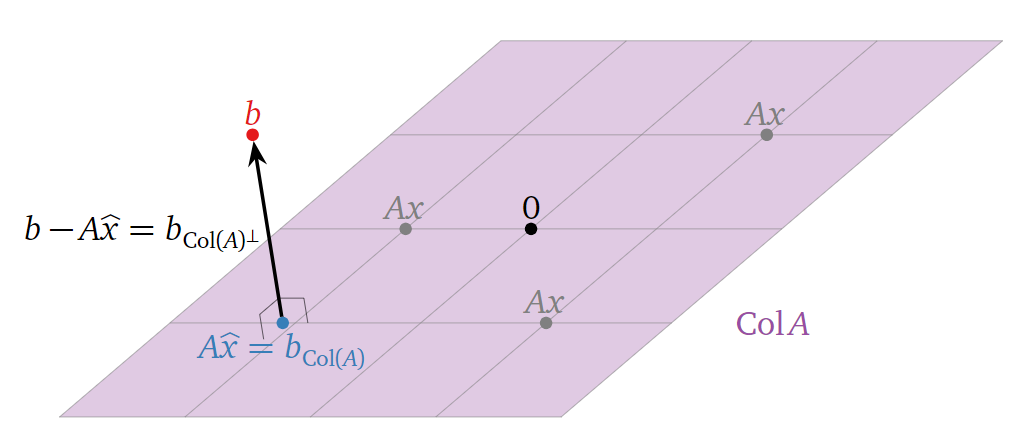
\includegraphics[width=1\linewidth]{image_2025-01-17_190701322.png}
    \caption{Obtenido de (The Method of Least Squares, n.d.)}
\end{wrapfigure}

\\

En la gráfica se aprecia la relación de ortogonalidad entre $b_{col(A)}$ y $b_{col(A)^\perp}$, que corresponden con la descomposición ortogonal de $b$ con respecto a $col(A)$. Esta es justo la cualidad que permite que $A\hat{x}$ sea el vector en $col(A)$ más cercano a $b$.
 
\\ Ahora, teniendo en cuenta lo demostrado, se tiene que $\hat{x}$ es la solución de la siguiente ecuación matricial:

$$ A^TA\hat{x} = A^Tb$$

Esto da una idea general de como solucionar un problema de mínimos cuadrados. A continuación se muestra un ejemplo:

\\ Con: $$A = \begin{bmatrix}
0 & 1 \\
1 & 1 \\
2 & 1
\end{bmatrix} \;\;\text{y} \;\; b = \begin{bmatrix} 6 \\ 0\\ 0 \end{bmatrix}$$

Halle la solución para el problema de mínimos cuadrados.

\\Solución: 

Primero, hallemos $A^T$, que corresponde a la matriz transpuesta:

$$A^T = \begin{bmatrix}
0 & 1 & 2\\
1 & 1 & 1 \\
\end{bmatrix}$$

Con esta, podrémos calcular el producto de matrices $A^TA$:

$$A^TA = \begin{bmatrix}
0 & 1 & 2\\
1 & 1 & 1
\end{bmatrix} \begin{bmatrix}
0 & 1 \\
1 & 1 \\
1 & 2
\end{bmatrix}  = \begin{bmatrix}
5 & 3 \\
3 & 3 \\
\end{bmatrix}$$

Por otro lado, $A^Tb$ también se calcula:

$$A^Tb = \begin{bmatrix}
0 & 1 & 2\\
1 & 1 & 1
\end{bmatrix}\begin{bmatrix} 6 \\ 0\\ 0 \end{bmatrix} =\begin{bmatrix} 0 \\ 6\\  \end{bmatrix} $$

De esta forma, se llega al siguiente sistema lineal de ecuaciones:

$$ \begin{bmatrix}
5 & 3 \\
3 & 3 \\
\end{bmatrix}\begin{bmatrix} \hat{x_1} \\ \hat{x_2}\\ \end{bmatrix} =\begin{bmatrix} 0 \\ 6\\  \end{bmatrix} $$

Cuya solución es: 
$$
\begin{bmatrix} \hat{x_1} \\ \hat{x_2}\\ \end{bmatrix} =\begin{bmatrix} -3 \\ 5\\  \end{bmatrix} $$
La visualización de la solución se puede ver a continuación:

\begin{wrapfigure}
    \centering
    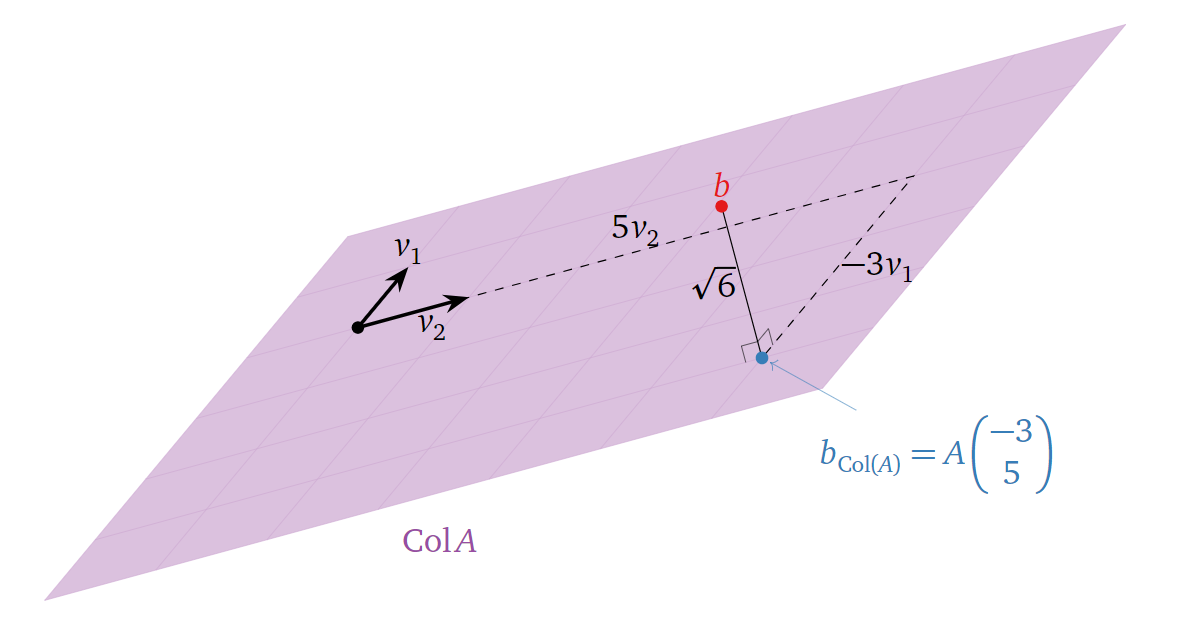
\includegraphics[width=1\linewidth]{image_2025-01-17_194708435.png}
    \caption{Obtenido de (The Method of Least Squares, n.d.)}
\end{wrapfigure}

En este caso, la distancia entre $b$ y $\hat{x}$ es de $\sqrt{6}$.


\section{Perspectiva desde el análisis de datos}

Una de las aplicaciones más importantes del método de mínimos cuadrados es dentro del ámbito de la Ciencia de los Datos. En específico, para calcular funciones que se aproximen al comportamiento de cierto conjunto de datos, es muy útil la aplicación de este método para encontra aquella función cuya distancia de los datos sea la más pequeña, por ejemplo

\\ Debido a la gran cantidad de aplicaciones existentes del método dentro de la Ciencia de los Datos, nos enfocaremos en el reconocido método de regresión lineal, que intenta hallar, dado un conjunto de datos de la forma $\{(x_i, y_i)_{i\in [1, n]}\}$, la función lineal $p(x) = a_1x \; + a_2$ cuya distancia a los datos sea mínima. 

\subsection{Regresión lineal}

Sea $\{(x_i, y_i)_{i\in [1, n]}\}$ un conjunto de datos donde $x$ es la variable independiente y $y$ es la variable dependiente de $x$. Se quiere ajustar los datos con una linea recta de la forma $p(x) = a_1x \;+ a_2$; esto es imposible al menos de que todos los puntos estén alineados. Por tanto, se busca una lína que minimice la siguiente cantidad:

$$S = \sum_{i = 1}^{n}(y_i - p(x_i))^2$$

Reemplazando $p(x_i)$ por $a_1x_i \; + a_2$, se obtiene que:

$$F(a_1,a_2) = \sum_{i = 1}^{n}(y_i - (a_1x_i \; + a_2))^2$$

Notemos que el proceso que se está realizando es un caso específico del proceso algebraico mostrado en la perspectiva algebraica; aquí, las funciones usadas para el ajuste son $f_1(x) = x $ y $ f_2(x) = 1$. 

\\Usando el resultado obtenido al final de la generalización de la perspectiva algebraica:
$$\begin{bmatrix}
    \sum_{i=1}^n(f_1(x_i))^2 & \sum_{k=1}^nf_1(x_i)f_2(x_i) &  \\
    \sum_{i=1}^nf_2(x_i)f_1(x_i) & \sum_{k=1}^n(f_2(x_i))^2 & 
 
\end{bmatrix}
\begin{bmatrix}
    c_1\\c_2\
\end{bmatrix} = \begin{bmatrix}
    \sum_{k=1}^n f_1(x_k)y_k\\\sum_{k=1}^n f_2(x_k)y_k
\end{bmatrix}$$

Se obtiene:

$$\begin{bmatrix}
    \sum_{i=1}^n(x_i)^2 & \sum_{k=1}^nx_i &  \\
    \sum_{i=1}^nx_i & n & 
 
\end{bmatrix}
\begin{bmatrix}
    c_1\\c_2\
\end{bmatrix} = \begin{bmatrix}
    \sum_{k=1}^nx_i y_i\\\sum_{k=1}^n y_i
\end{bmatrix}$$


De aquí, se pueden obtener las soluciones para $a_1 $ y $a_2$. Notar que, para otro ajuste que no sea necesariamente lineal, el uso de la fórmula generalizada sirve como insumo para llegar al sistema de ecuaciones lineales cuya solución proveer los coeficientes $a_i$. Para el caso del código de nuestro caso, se analizan distintos ajustes posibles para obtener, como polinomios de distintos grados, hasta obtener una solución que, sin problemas de overfitting, genere el error residual más pequeño.

% Referencias
%%%%%%%%%%%%%%%%%%%%%%%%%%%%%%%%%%%%

\section{Referencias}
\begingroup
\renewcommand{\section}[2]{}
\begin{thebibliography}{0}
\setlength{\parskip}{0mm}
\setlength{\itemsep}{-0.3mm}
\small

\bibitem{WikipediaLeastSquares} Wikipedia, \textit{Least squares}, 
\textit{Wikipedia, The Free Encyclopedia}, 
Available at: \url{https://en.m.wikipedia.org/wiki/Least_squares}, 
Accessed on: January 5, 2025.

\bibitem{LeastSquaresMethodUnipv} University of Pavia, \textit{Least squares method}, 
\textit{}
Available at: \url{https://www-dimat.unipv.it/sangalli/numerical_methods_eng_sciences/10%20-%20Least%20Squares.pdf}, 
Accessed on: January 17, 2025.

\bibitem{LeastSquaresMethodMargalit,Rabinoff} Interactive Linear Algebra, \textit{Orthogonal projection}, 
\textit{}
Available at: \url{https://textbooks.math.gatech.edu/ila/projections.html}, 
Accessed on: January 17, 2025.


\end{thebibliography}
\endgroup

\end{document}
